%%%%%%%%%%%%%%%%%%%%%%%%%%%%%%%%%%%%%%%%%
% Short Sectioned Assignment
% LaTeX Template
% Version 1.0 (5/5/12)
%
% This template has been downloaded from:
% http://www.LaTeXTemplates.com
%
% Original author:
% Frits Wenneker (http://www.howtotex.com)
%
% License:
% CC BY-NC-SA 3.0 (http://creativecommons.org/licenses/by-nc-sa/3.0/)
%
%%%%%%%%%%%%%%%%%%%%%%%%%%%%%%%%%%%%%%%%%

%----------------------------------------------------------------------------------------
%	PACKAGES AND OTHER DOCUMENT CONFIGURATIONS
%----------------------------------------------------------------------------------------

\documentclass[paper=a4, fontsize=11pt]{scrartcl} % A4 paper and 11pt font size

\usepackage[T1]{fontenc} % Use 8-bit encoding that has 256 glyphs
\usepackage{fourier} % Use the Adobe Utopia font for the document - comment this line to return to the LaTeX default
\usepackage[english]{babel} % English language/hyphenation
\usepackage{amsmath,amsfonts,amsthm} % Math packages

\usepackage{graphicx}

\usepackage{sectsty} % Allows customizing section commands
\allsectionsfont{\centering \normalfont\scshape} % Make all sections centered, the default font and small caps

\usepackage{subcaption}
\usepackage{pdfpages}
\usepackage{float}

\usepackage{fancyhdr} % Custom headers and footers
\pagestyle{fancyplain} % Makes all pages in the document conform to the custom headers and footers
\fancyhead{} % No page header - if you want one, create it in the same way as the footers below
\fancyfoot[L]{} % Empty left footer
\fancyfoot[C]{} % Empty center footer
\fancyfoot[R]{\thepage} % Page numbering for right footer
\renewcommand{\headrulewidth}{0pt} % Remove header underlines
\renewcommand{\footrulewidth}{0pt} % Remove footer underlines
\setlength{\headheight}{13.6pt} % Customize the height of the header

\numberwithin{equation}{section} % Number equations within sections (i.e. 1.1, 1.2, 2.1, 2.2 instead of 1, 2, 3, 4)
\numberwithin{figure}{section} % Number figures within sections (i.e. 1.1, 1.2, 2.1, 2.2 instead of 1, 2, 3, 4)
\numberwithin{table}{section} % Number tables within sections (i.e. 1.1, 1.2, 2.1, 2.2 instead of 1, 2, 3, 4)

\setlength\parindent{0pt} % Removes all indentation from paragraphs - comment this line for an assignment with lots of text

%----------------------------------------------------------------------------------------
%	TITLE SECTION
%----------------------------------------------------------------------------------------

\newcommand{\horrule}[1]{\rule{\linewidth}{#1}} % Create horizontal rule command with 1 argument of height

\title{	
\normalfont \normalsize 
\textsc{Bonn-Rhein-Sieg University of Applied Sciences} \\ [25pt] % Your university, school and/or department name(s)
\horrule{0.5pt} \\[0.4cm] % Thin top horizontal rule
\huge Scientific Experimentation and Evaluation\\
- Assignment 02 - \\ 
Experiment Report \\% The assignment title
\horrule{2pt} \\[0.5cm] % Thick bottom horizontal rule
}

\author{Mazin Eltayeb, Bastian Lang} % Your name

\date{\normalsize\today} % Today's date or a custom date

\begin{document}

\maketitle % Print the title

\tableofcontents
\newpage

\section{Abstract}
% Especially how to mark positions, how to ensure identical start postitions
% Program and Parameters used to drive the robot
% Any observation made during the execution, that may help to understand the outcome of the experiments
This report describes the performance of some experiments to measure the motion of a Lego robot.
It describes the robot used, the measurement process, the performance of the experiment and its results.



\section{The Robot's Design}
% Description and Picture of the Robot (best front, side and top view
% Information about parameters like wheel diameter, wheel distance, marker positions
Our robot is the 5-minutes bot from the official Lego website with some additions made (see figure \ref{fig:robot}. 
It has the standard two actuated wheels to the left and the right of the robot and one fixed non-actuated wheel in the back. 
The actuated wheels have a diameter of 5.6cm and are each about 8.5cm displaced with respect to the center. 
Right next to its actuated wheels are two markers close to the ground aligned with the wheel axis to be used to measure the position of the robot.

\begin{figure}[H]
 
\begin{subfigure}{0.5\textwidth}
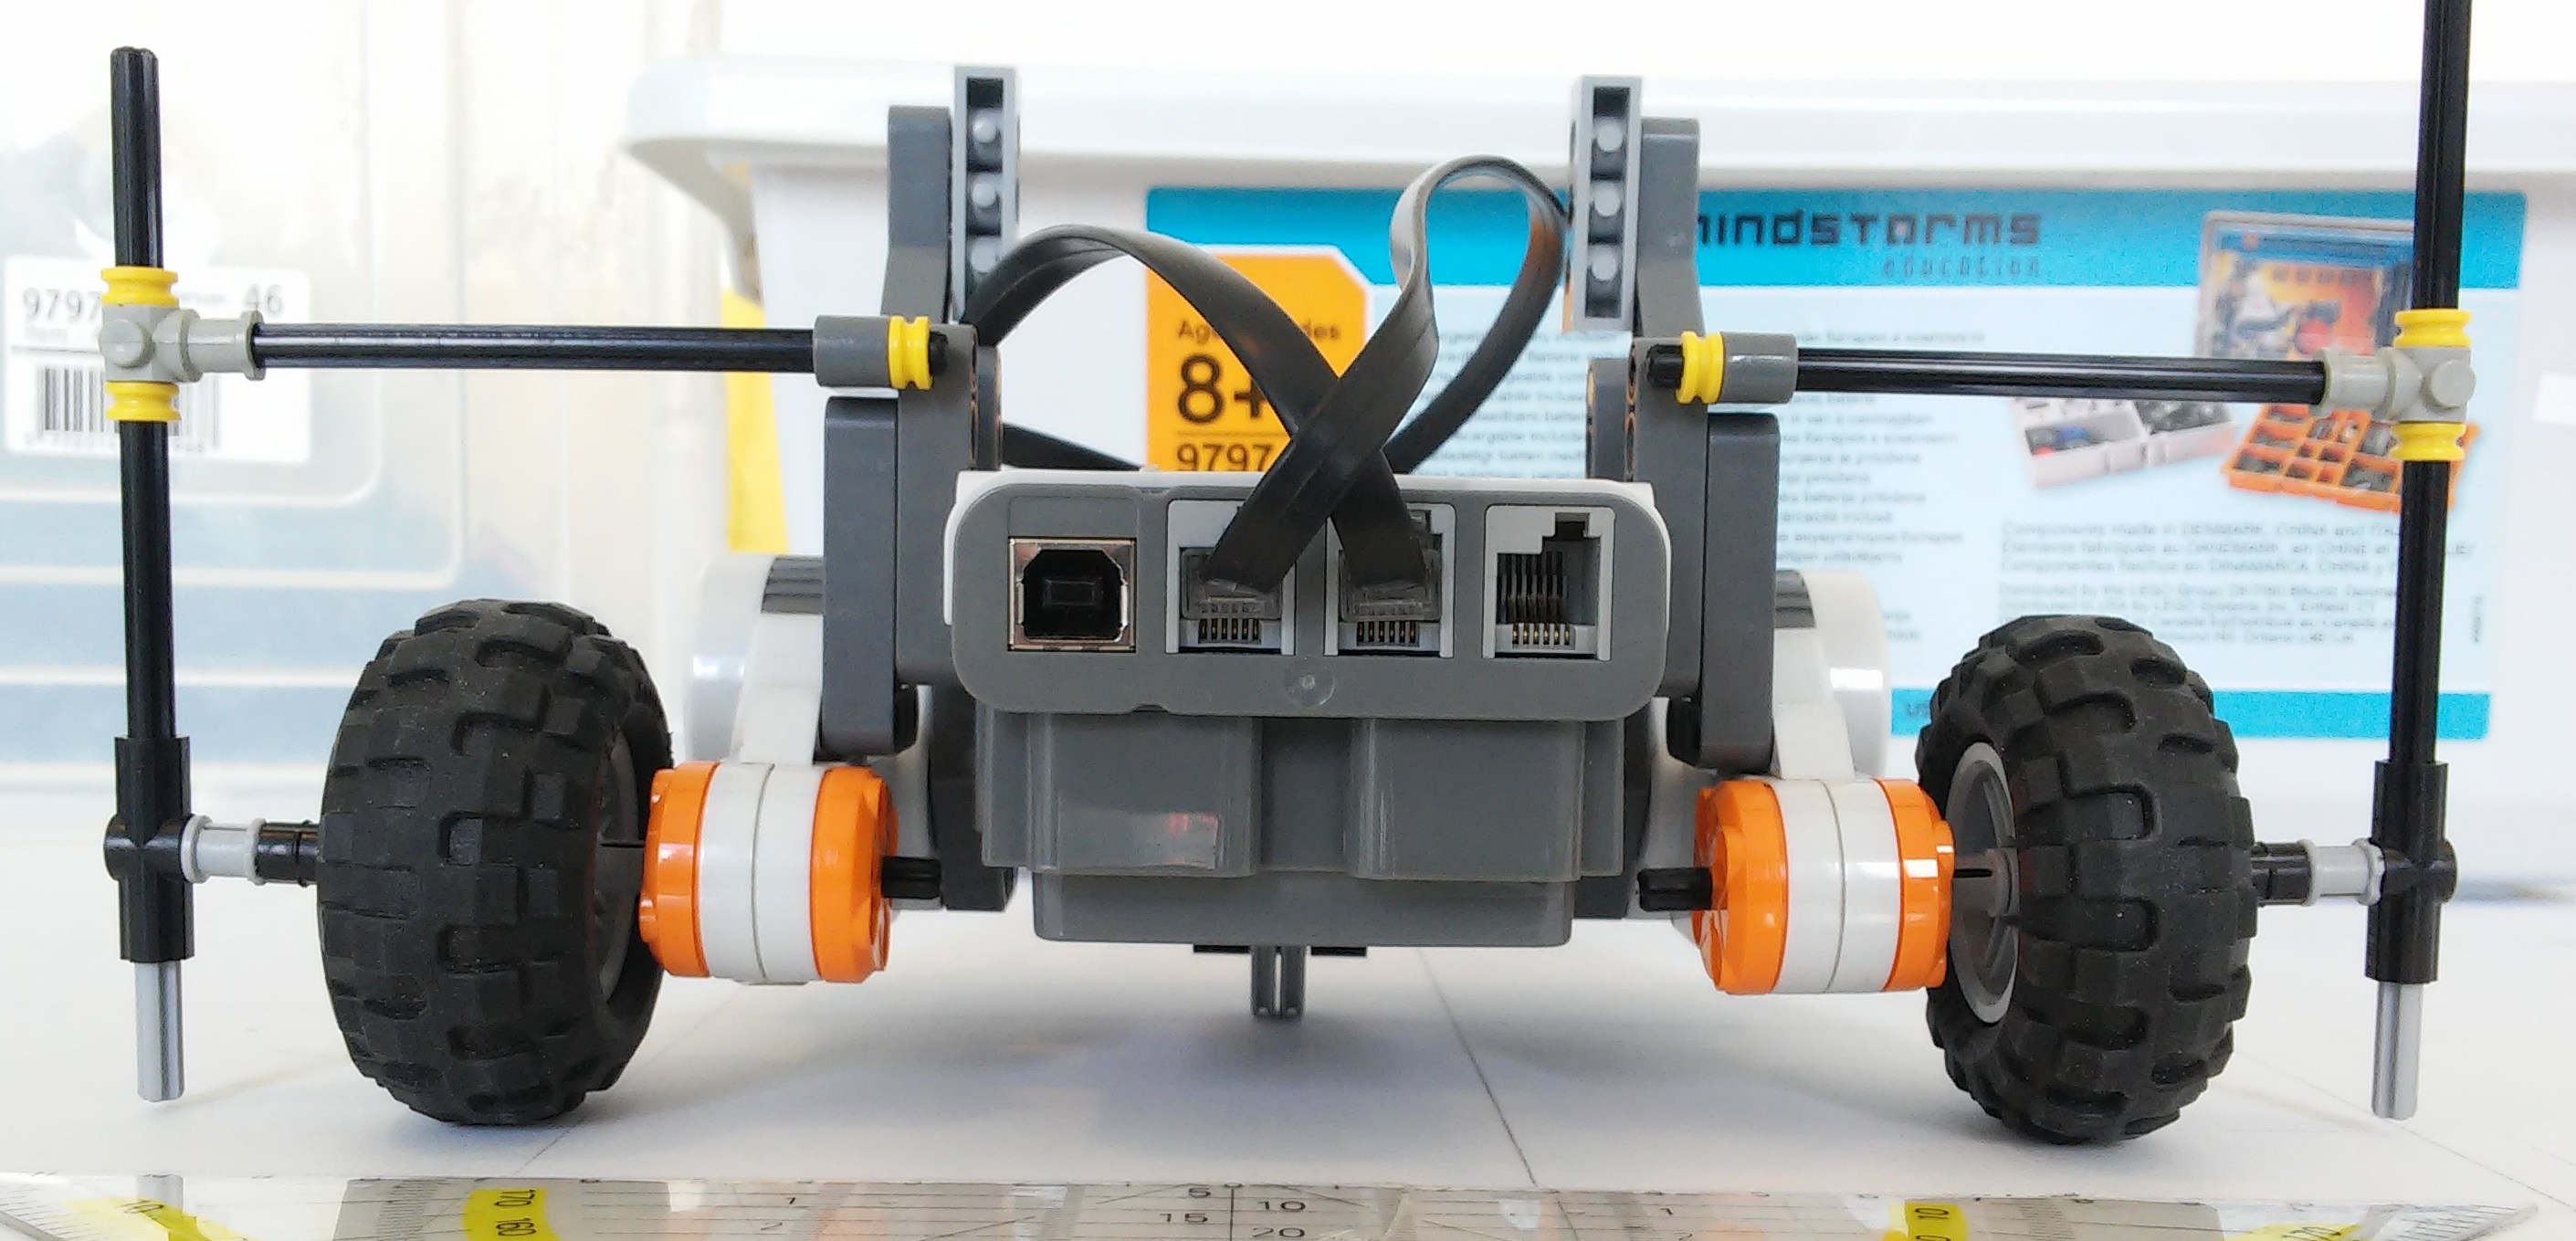
\includegraphics[width=0.9\linewidth, height=5cm]{front.png} 
\caption{Front View}
\label{fig:sub_front}
\end{subfigure}
\begin{subfigure}{0.5\textwidth}
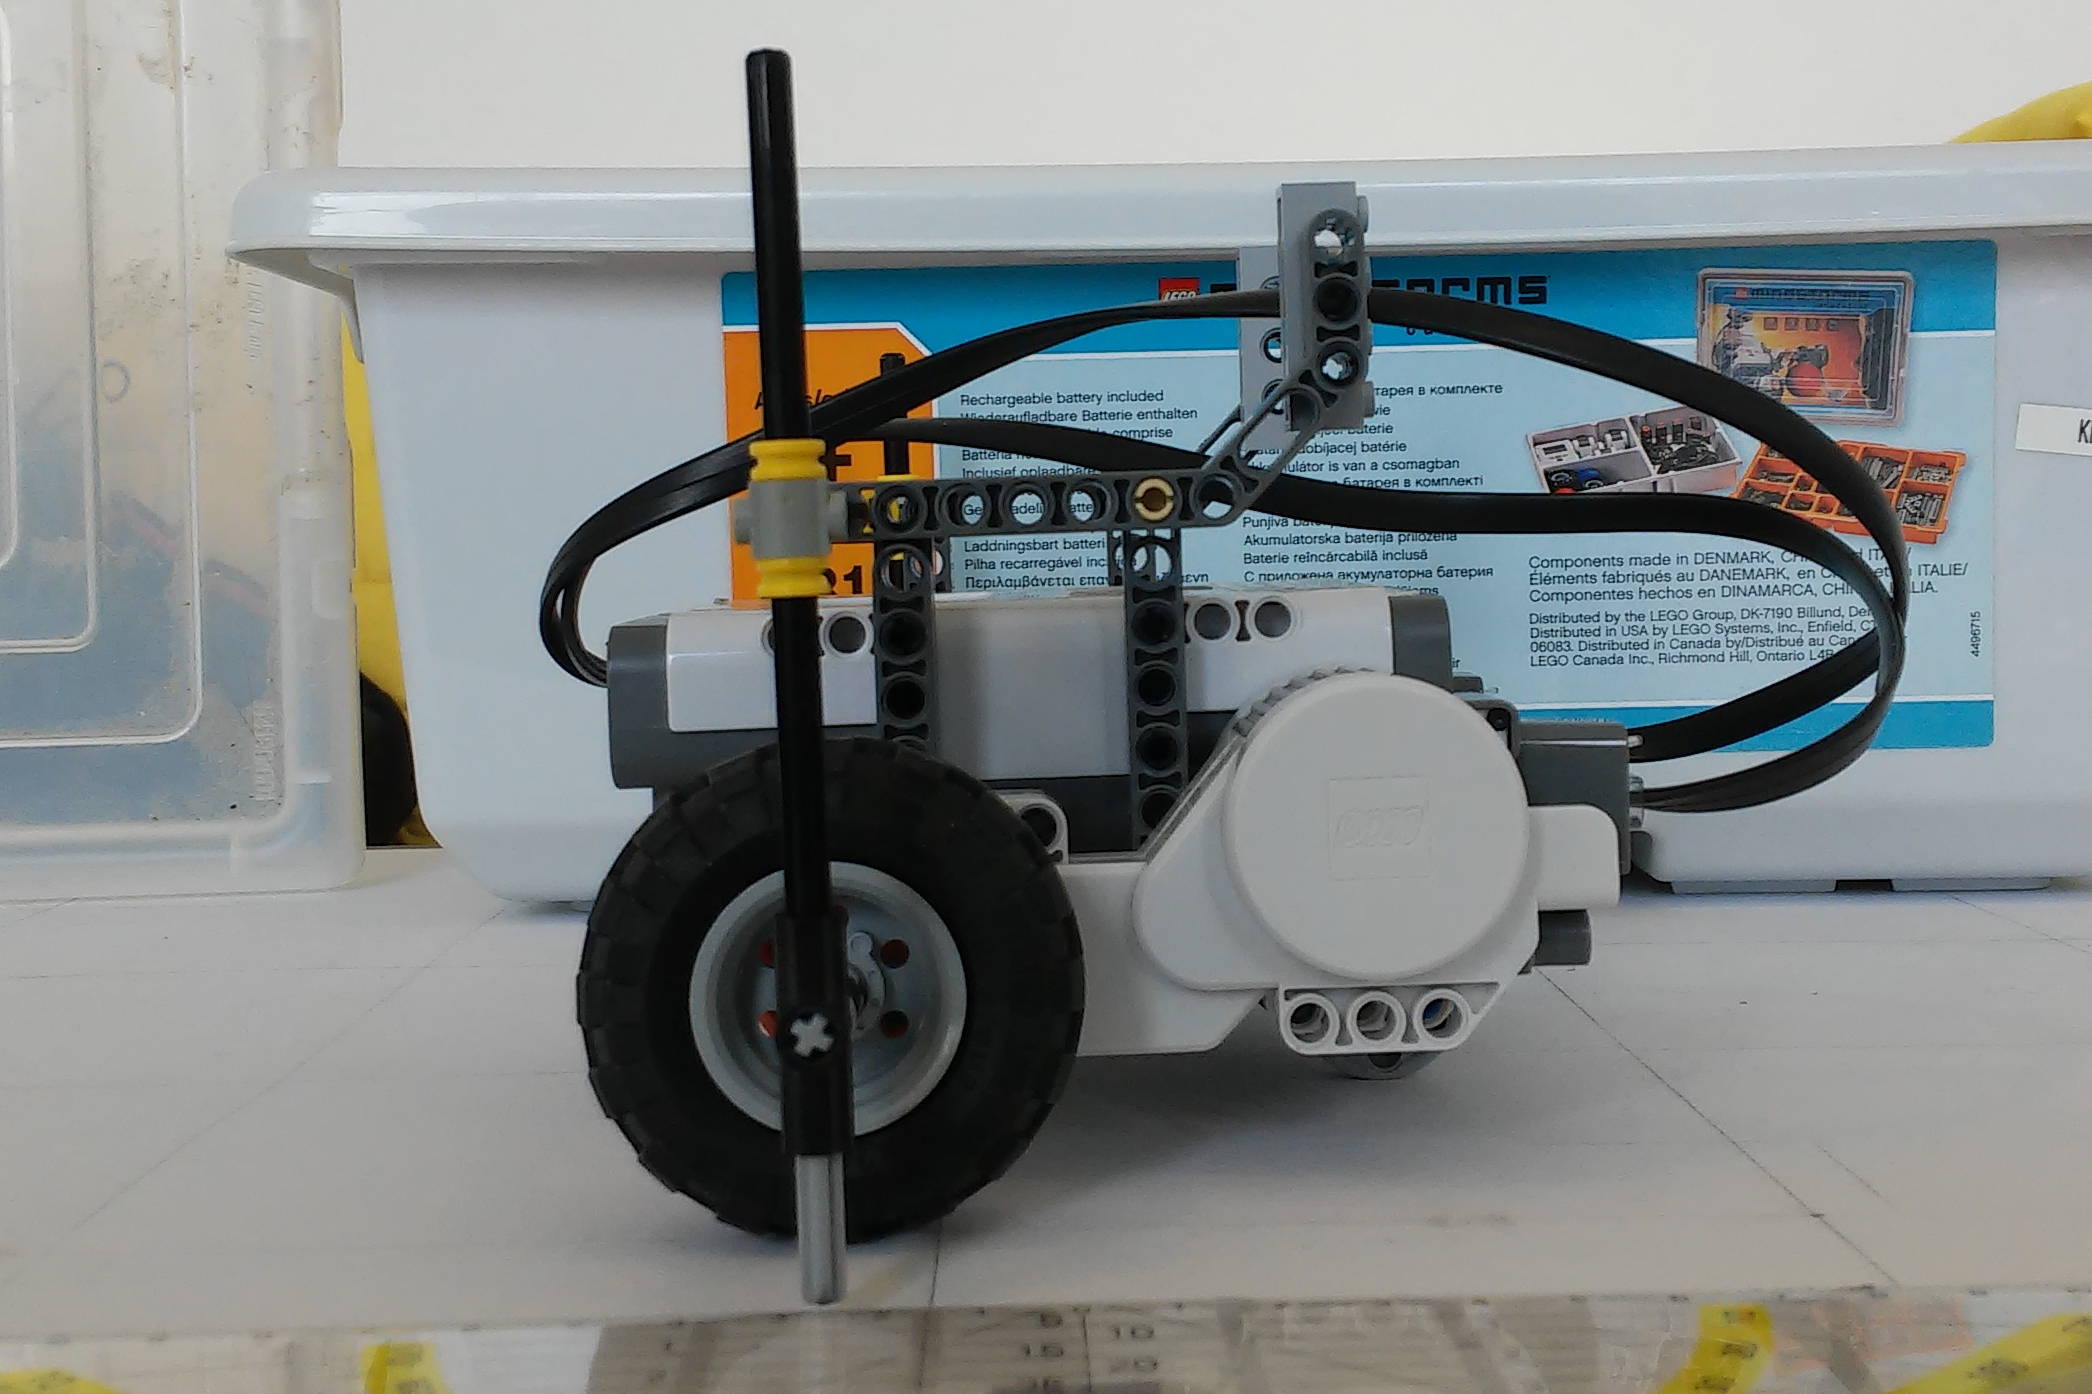
\includegraphics[width=0.9\linewidth, height=5cm]{side.png}
\caption{Side View}
\label{fig:sub_side}
\end{subfigure}
\begin{subfigure}{0.5\textwidth}
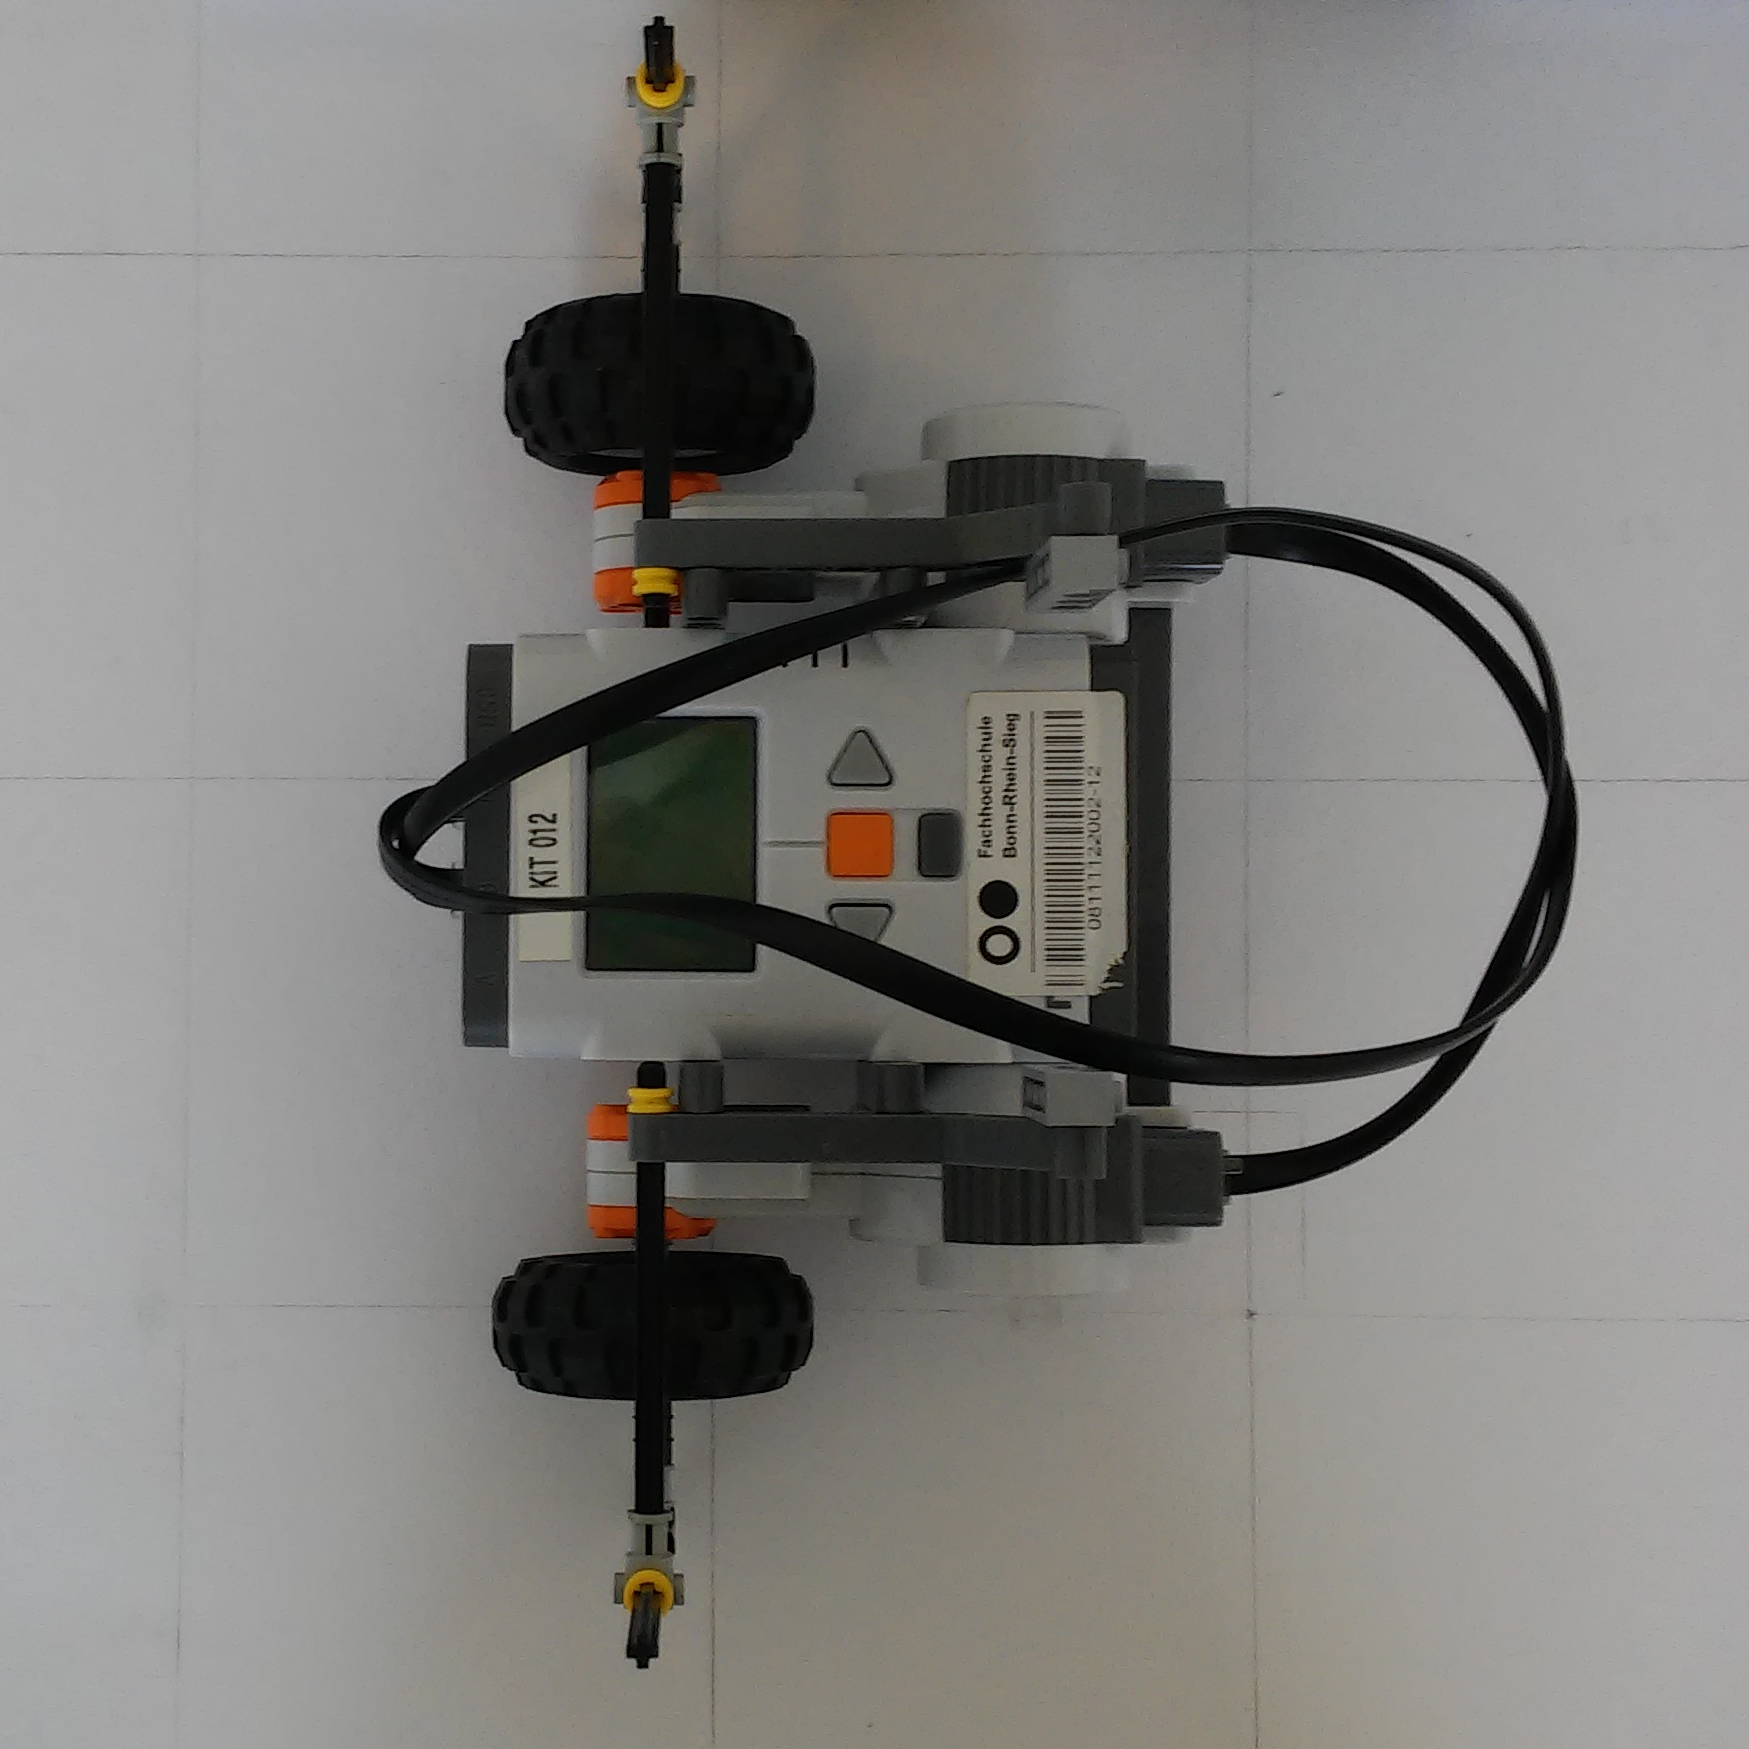
\includegraphics[width=0.9\linewidth, height=5cm]{top.png}
\caption{Top View}
\label{fig:sub_top}
\end{subfigure}
 
\caption{Images of the robot}
\label{fig:robot}
\end{figure}


\section{The Measurement Process}
% How to use the marker to mark positions, how to use the grid and rulers to measure positions
% Coordinate origin
% Picture of grid
% Picture of marking a pose
On our measurement facility we mark the starting positions of the two markers on the ground and define the position of the right marker as the origin of our grid. 
The y-axis points in the direction the robot is facing and the x-axis to the right.
The experiments consists of three parts:
\begin{itemize}
	\item Driving forward
	\item Right Arc
	\item Left Arc
\end{itemize}
Before performing the drive command, we place the robot in the start position and manually align its markers with the marks on the ground.
After performing the drive command we press the markers down so the touch the ground and mark their positions with a sharpened pencil.
We then use rulers to measure the positions of the marks with respect to the origin of our system.
After each run we erase all but the start markers and place the robot the back at the start position.
We repeat this 20 times for each experiment.
During all the experiments the robot is plugged to the power source.

\begin{figure}[H]
 
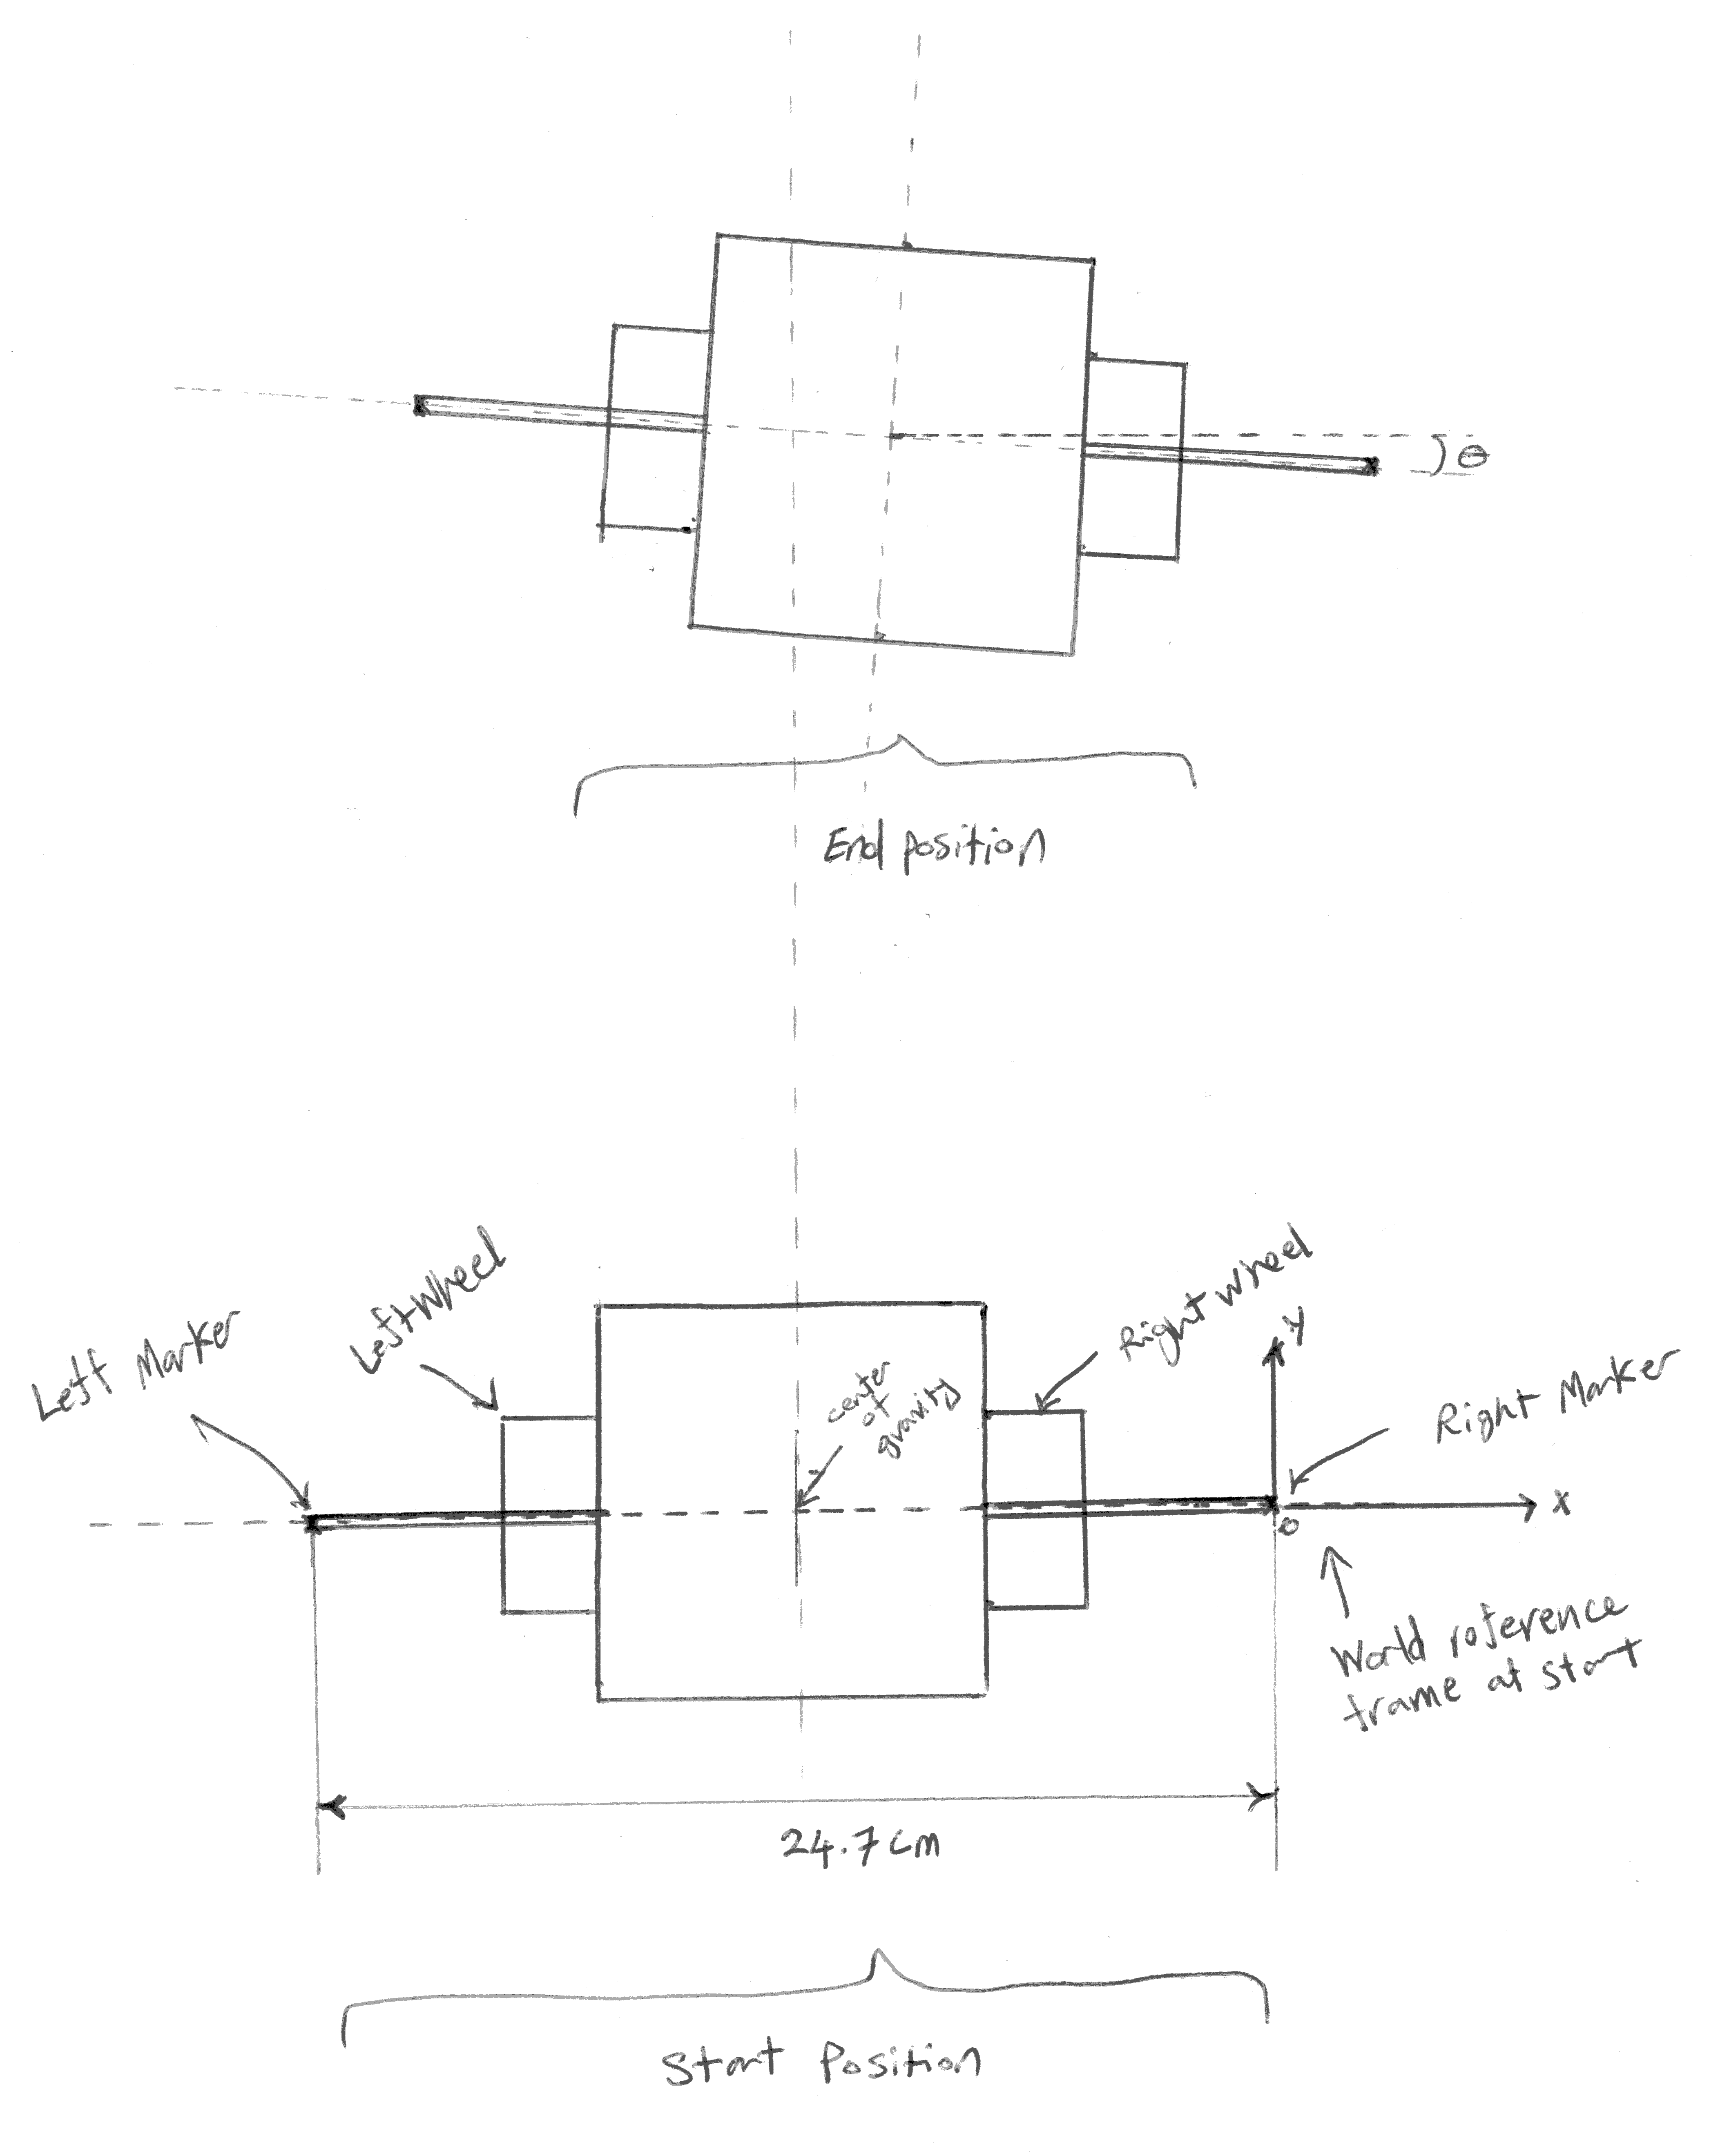
\includegraphics[width=0.9\linewidth]{experimental_setup.png} 
\caption{Sketch of Experiment Performance}
\label{fig:setup}
\end{figure}


\section{Experiment}
% General description
We tested three different scenarios for driving the robot.
The first was to let the robot drive forward by letting the wheels do 1.5 rotations with full power.
The second was driving in a right arc by commanding the left wheel to do 2 rotations with full power and the right wheel to do 1 rotation with half power.
The last scenario was driving in a left arc by rotating the left wheel once with half power and the right wheel twice with full power.
The programs created in Lego's visual IDE can be seen in figure \ref{fig:code}

\begin{figure}[H]
 
\begin{subfigure}{0.5\textwidth}
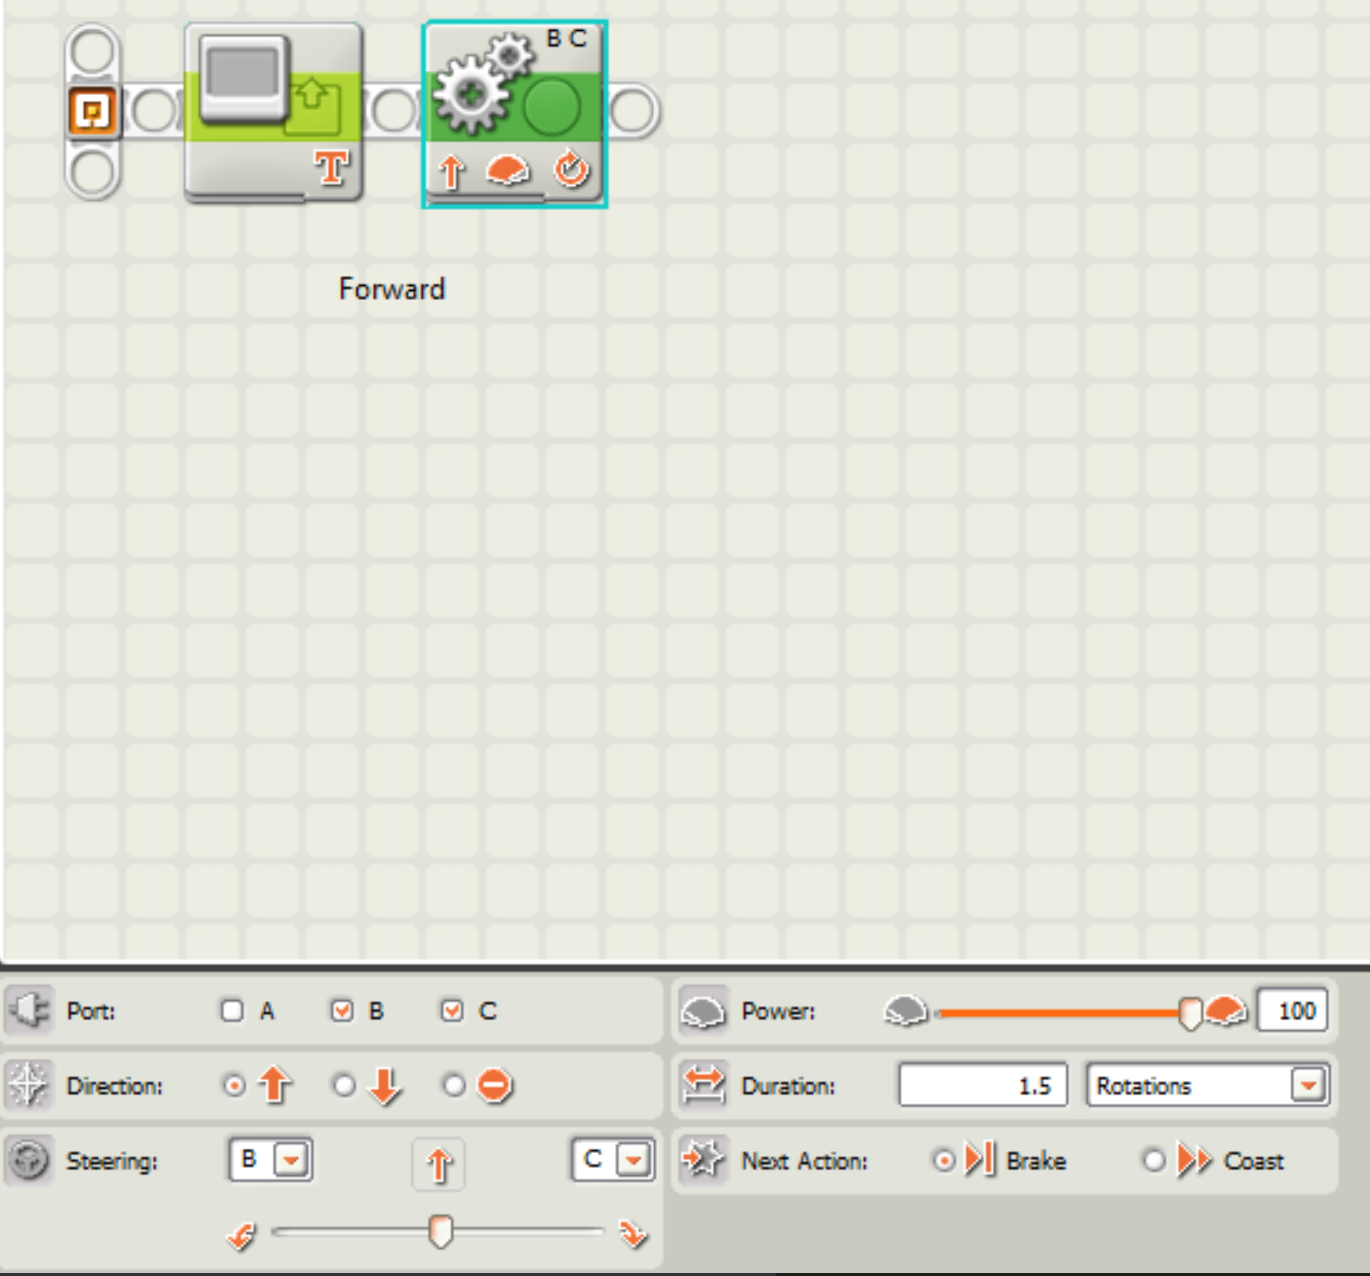
\includegraphics[width=0.9\linewidth, height=5cm]{forward_code.PNG} 
\caption{Program for forward motion}
\label{fig:sub_forward_code}
\end{subfigure}
\begin{subfigure}{0.5\textwidth}
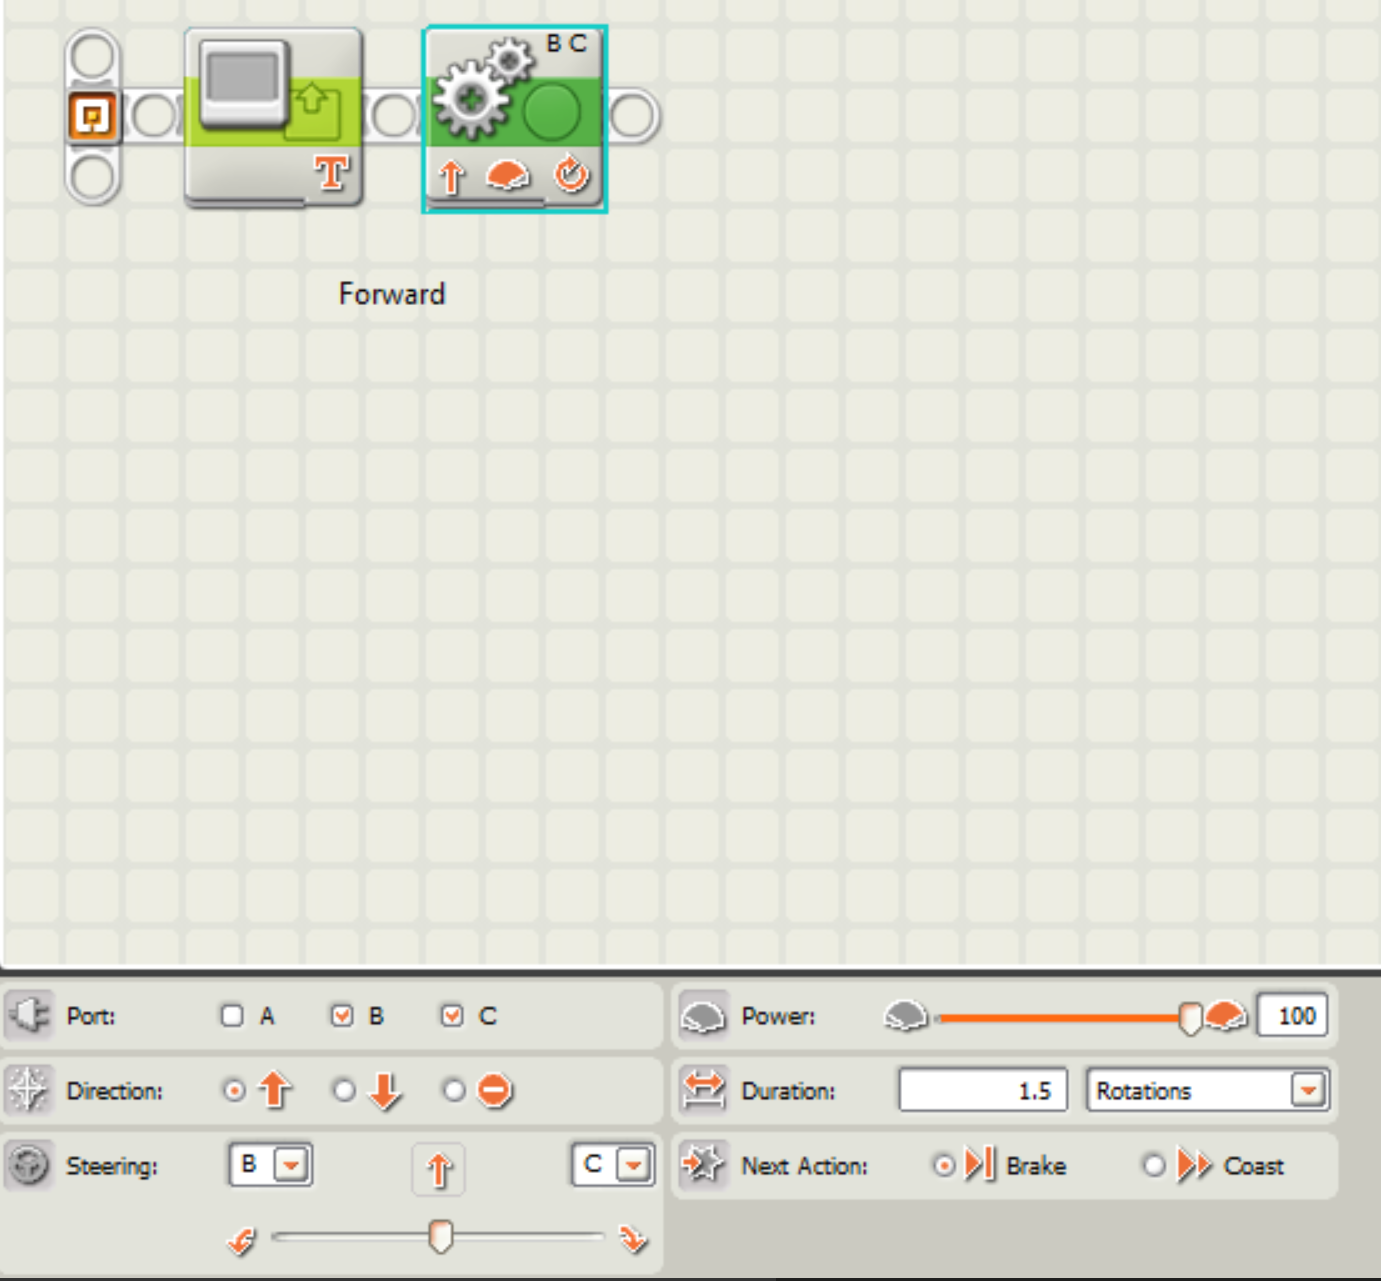
\includegraphics[width=0.9\linewidth, height=5cm]{right_arc_code.PNG}
\caption{Program for Right Arc}
\label{fig:sub_right_code}
\end{subfigure}
\begin{subfigure}{0.5\textwidth}
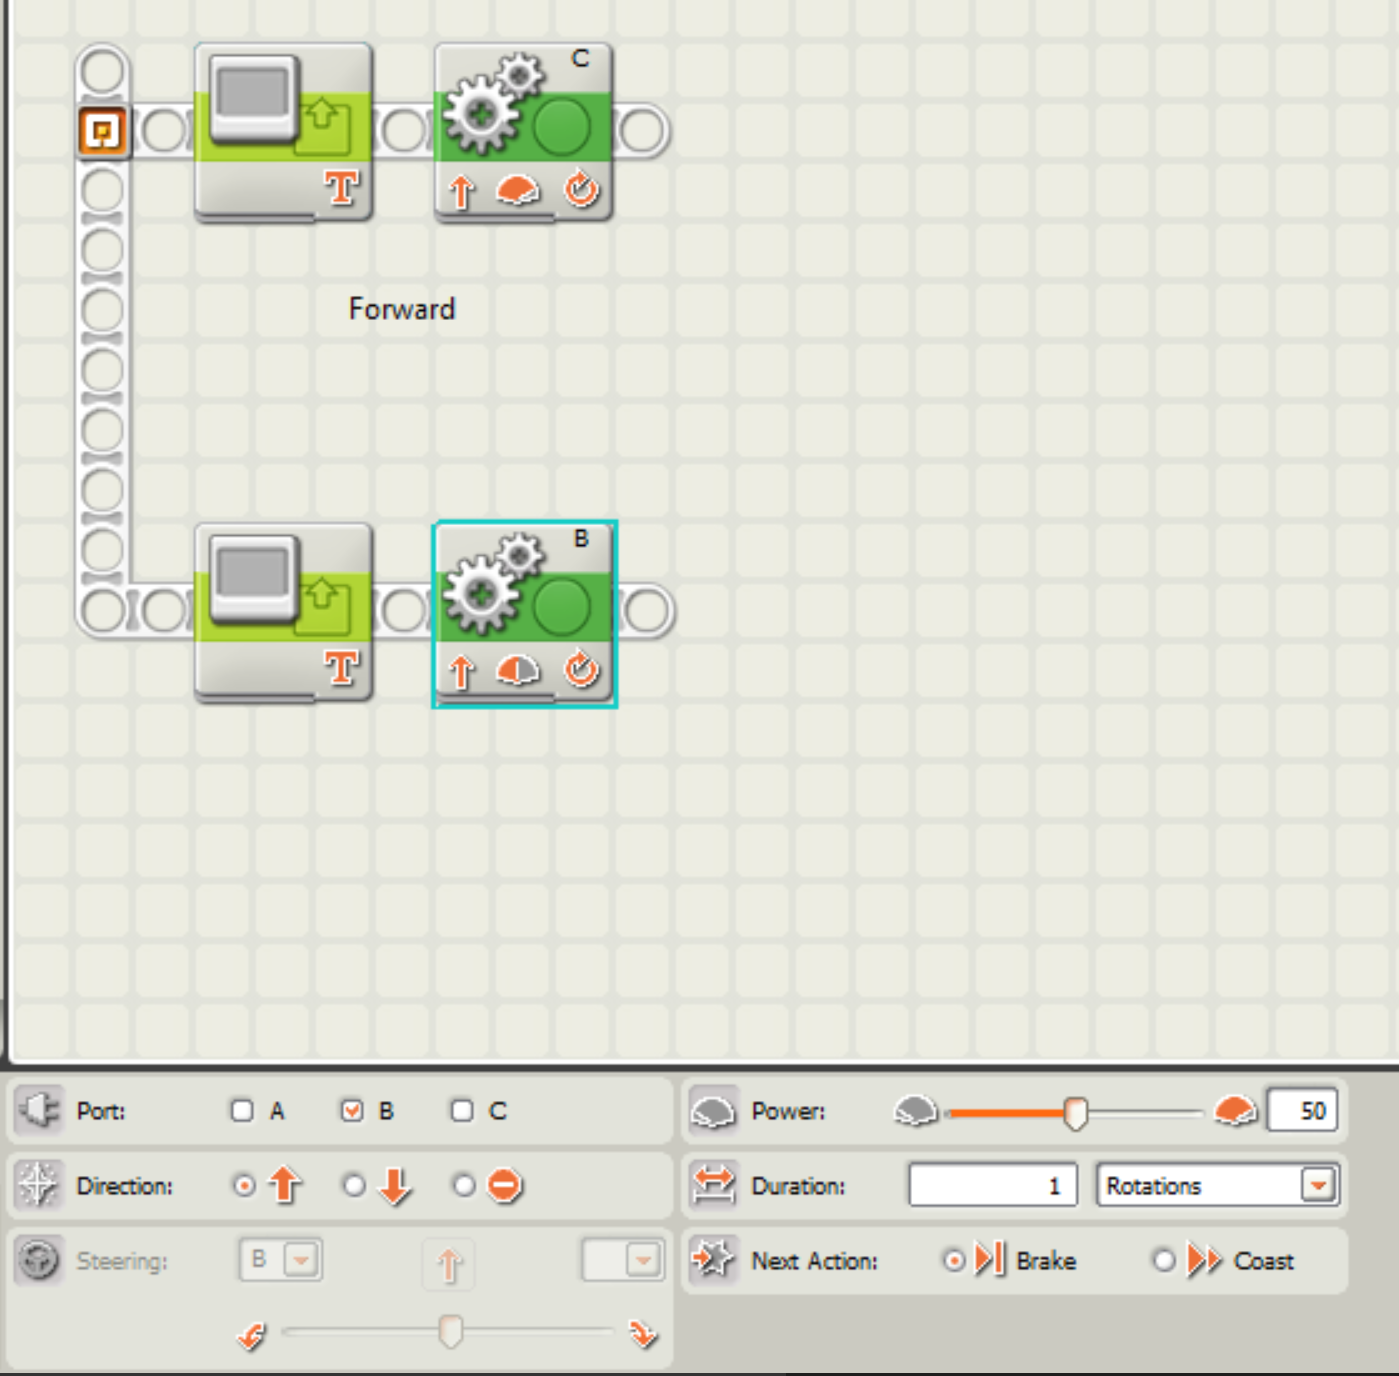
\includegraphics[width=0.9\linewidth, height=5cm]{left_arc_code.PNG}
\caption{Program for Left Arc}
\label{fig:sub_left_code}
\end{subfigure}
 
\caption{Programs used for the experiments in Lego's visual IDE}
\label{fig:code}
\end{figure}

\section{Results}
% Tables of positions (maybe sheets are sufficient)
% Plot of 2D coordinates
The results of the experiments can be seen in the appendix (Section \ref{sec:appendix}).




\subsection{Forward}
Given a straight movement with 5.6cm wheel diameter and 1.5 rotations we would expect a travelled distance of about 26.4cm.
The average in our experiments is 24.8cm for the left wheel and 24.0 for the right wheel.
The final orientation was tilted by minus two degrees in average with a standard deviation of 2 degrees.


\subsection{Right Arc}
For the right arc the left wheel's final position was in average (-8.4|32.0) with a standard deviation of (0.5cm|0.2cm).
The right wheel's final position was (5.2|11.4) in average with a standard deviation of (0.3cm|0.3cm).
The final orientation was -56 degrees in average with a standard deviation of 1.

\subsection{Left Arc}
For the right arc the left wheel's final position was in average (-30.8|11.5) with a standard deviation of (0.1cm|0.2cm).
The right wheel's final position was (-16.1|31.5) in average with a standard deviation of (0.3cm|0.2cm).
The final orientation was 54 degrees in average with a standard deviation of 1.

\section{Conclusion}
For the straight forward experiment we expected more travelled distance and no tilting in the end, but the robot was slightly tilted to the right in average.
For the arc-experiments we expected a similar, but negated result than the opposite movement.
But it turned out that the robot was turning slightly more to the right than to the left.
Overall we could observe a small bias to the right.


\begin{figure}[H]
 
\begin{subfigure}{0.5\textwidth}
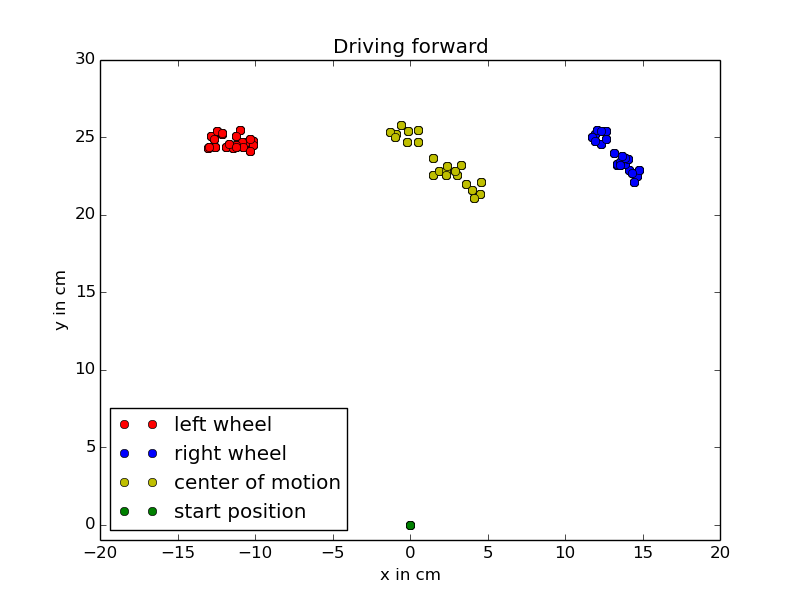
\includegraphics[width=0.9\linewidth, height=5cm]{forward.png} 
\caption{Driving forward}
\label{fig:sub_forward}
\end{subfigure}
\begin{subfigure}{0.5\textwidth}
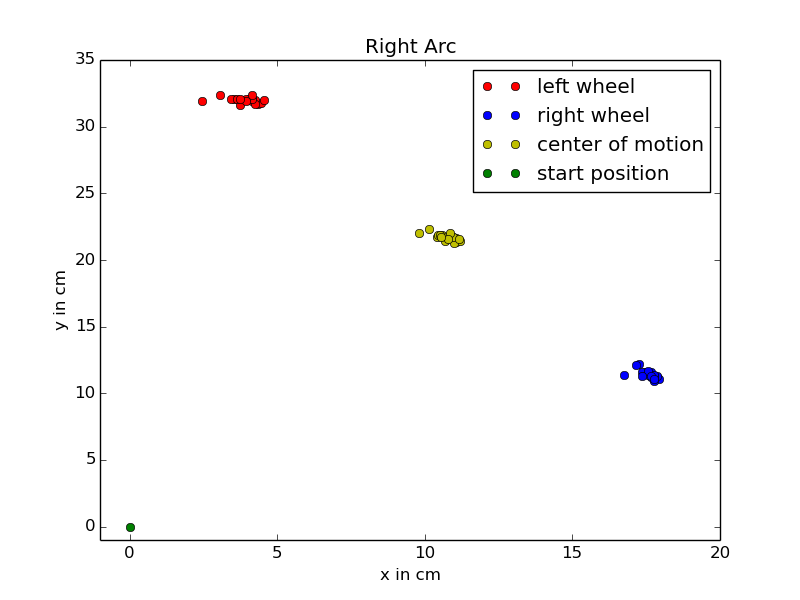
\includegraphics[width=0.9\linewidth, height=5cm]{right_arc.png}
\caption{Right Arc}
\label{fig:sub_right}
\end{subfigure}
\begin{subfigure}{0.5\textwidth}
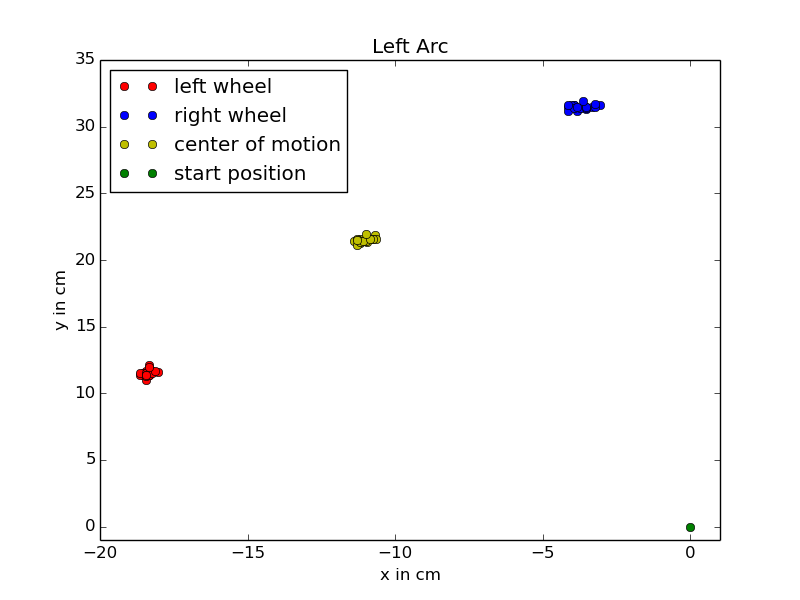
\includegraphics[width=0.9\linewidth, height=5cm]{left_arc.png}
\caption{Left Arc}
\label{fig:sub_left}
\end{subfigure}
 
\caption{Plots of robot's end positions}
\label{fig:plots}
\end{figure}

\section{Appendix}
\label{sec:appendix}
%\begin{figure}[h]
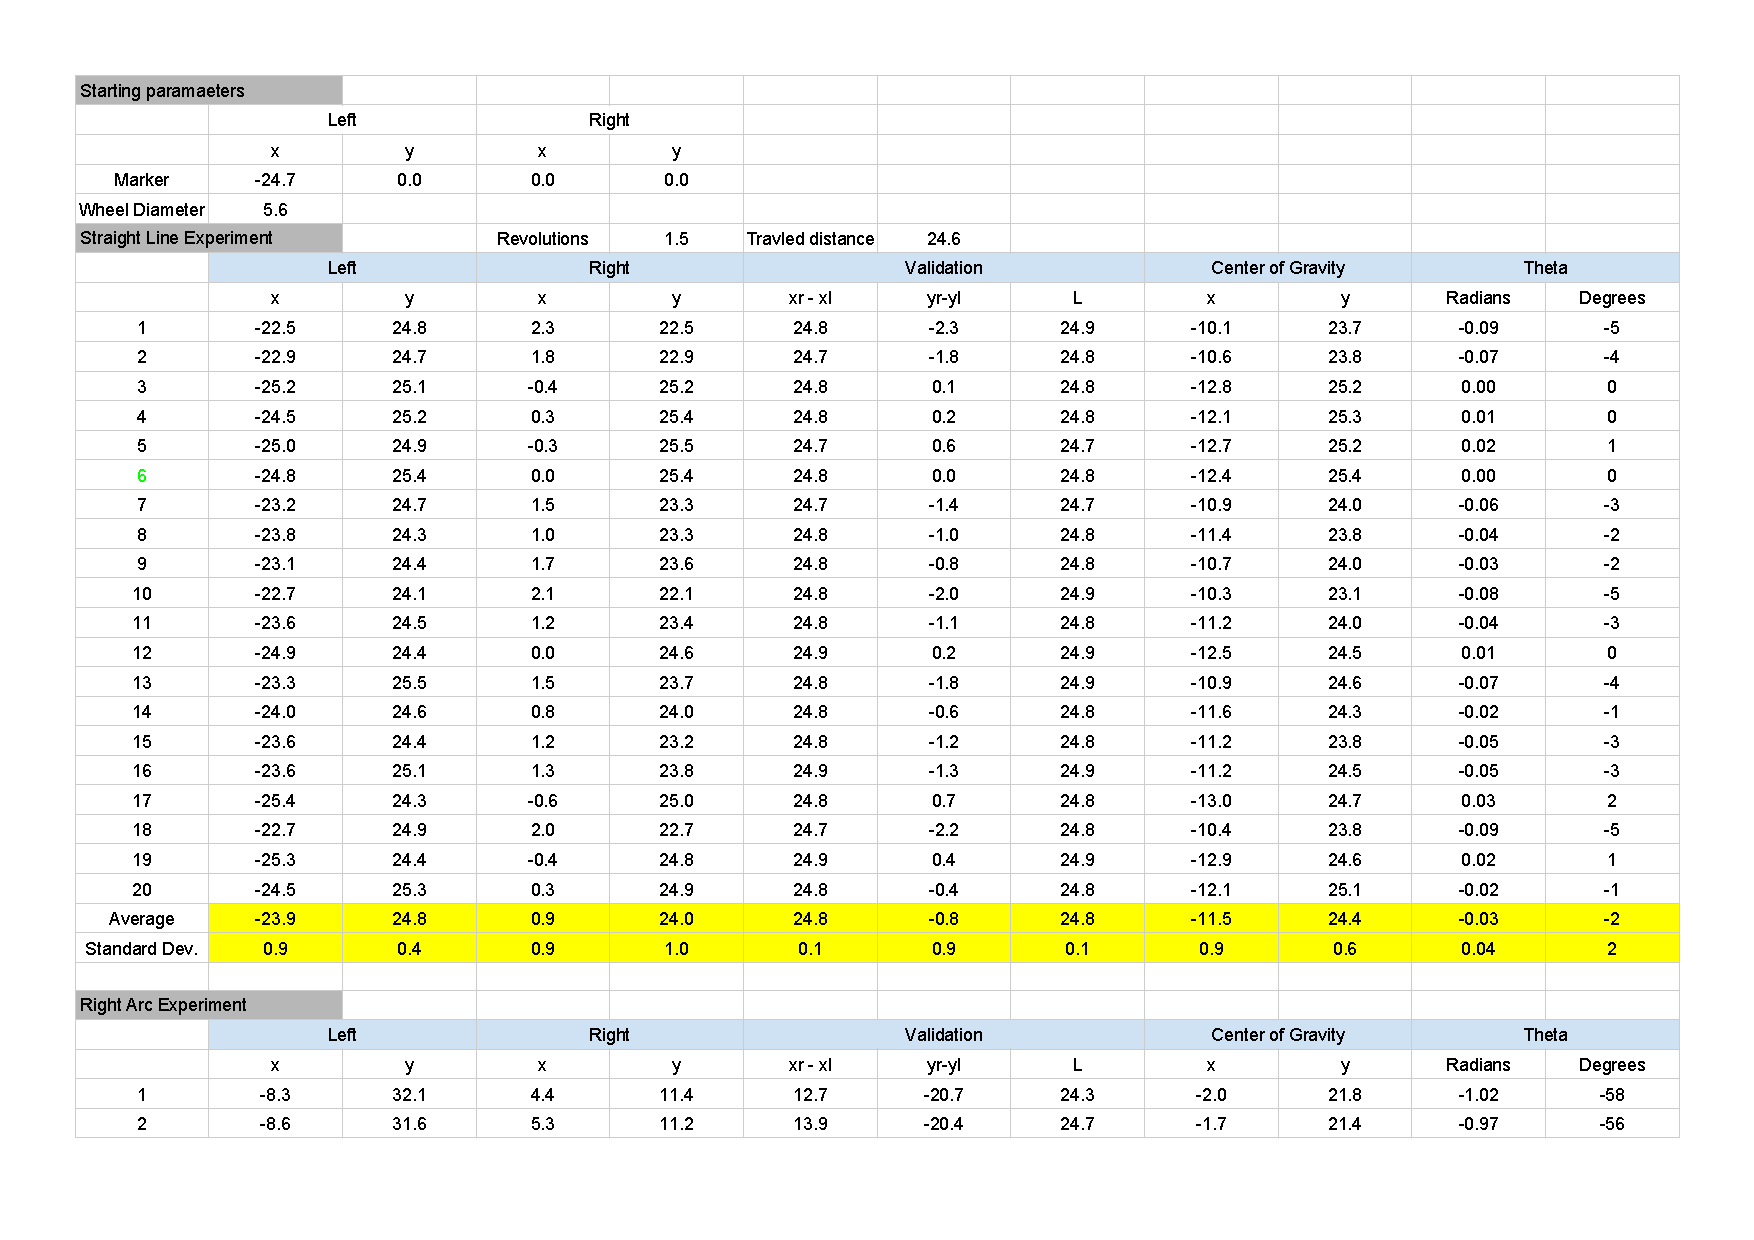
\includepdf[pages={1,2,3}]{final_results.pdf}
%\caption{Data Table of the Experiments}
%\label{fig:data}

%\end{figure}













\end{document}